\motto{}
\chapter{Pervasive Concepts}
\label{intro03} % Always give a unique label
% use \chaptermark{}
% to alter or adjust the chapter heading in the running head

\abstract{
}

\section{Characteristics}
\label{sec:03:1}

Characteristics are containers that record a set of attribute values
(ex: number\_of\_drivers = 2, make\_of\_car = Honda, resale\_value=10000)
which a policy contract is based on, and additionally a time interval over which
those attribute values are valid. Abstractly, it's a combination of a map and a time
interval. 

Below we just consider the time interval part of a characteristics and detail
how those intervals split as the standard modification operations are applied
to intervals
\import{ch03/}{CharacteristicsSplitCtx0-sa.tex}
\import{ch03/}{CharacteristicsSplitMch0-sa.tex}

\section{Liquid Calculations}
\label{sec:03:2}

\import{ch03/}{CancellationCalculations-sa.tex}

\section{Intervals}
As you work with framework objects, you will soon come to see that most objects cover
an interval from $start\_timestamp$ to $end\_timestamp$. These times delineate an extent of
a coverage interval or in the case of a modification the times delineate the time range for
which a coverage change was requested.

There is also a second type of framework object which is very common and interval like. These
are temporal objects and are identifiable by the fields $issued\_timestamp$ and $replaced\_timestamp$.
More commonly you may have seen these fields in other frameworks by the names $valid\_from$ and
$valid\_to$. This simple structure is used to record an audit history and allow easy acquisition of the current set
of valid objects with a filter of the form
\begin{equation*}
issuedTimestamp \neq null \land replacedTimestamp = null
\end{equation*}

Here are some standard interval functions that are available for use in the framework.
\import{ch03/}{IntervalOps-sa.tex}

\section{Holdbacks}
\label{sec:03:3}

\subsection{Concept}

\begin{figure}[ht]
  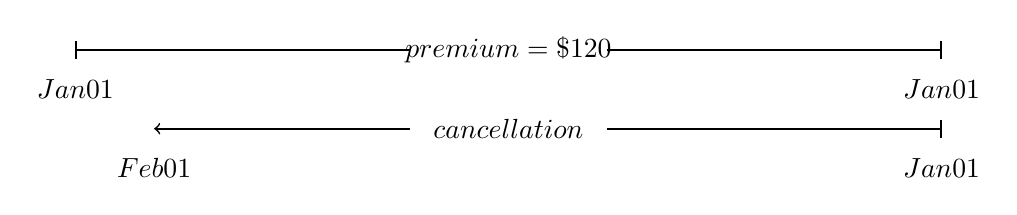
\begin{tikzpicture}
    \draw[|-,semithick] (0,-0.5) -- (4.25,-0.5);
    \draw (5.5, -0.5) node {$premium = \$120$};
    \draw[-|,semithick] (6.75,-0.5) -- (11,-0.5);
    \draw (0,-1) node {$Jan 01$};
    \draw (11,-1) node {$Jan 01$};
    
    \draw[<-,semithick] (1,-1.5) -- (4.25,-1.5);
    \draw (5.5, -1.5) node {$cancellation$};
    \draw[-|,semithick] (6.75,-1.5) -- (11,-1.5);
    \draw (1,-2) node {$Feb 01$};
    \draw (11,-2) node {$Jan 01$};
    
  \end{tikzpicture}   
  \caption{
    A policy and a cancellation
  }
  \label{fig:3:1}
\end{figure}

To explain holdbacks consider a policy running from Jan 1st of one year to Jan 1st of the next year, with a
premium of 120 dollars. If
a customer decided to cancel this policy starting at Feb 1st, then there are two adjustments that would
be made to this policy. First the premium would be prorated to account for the single month of coverage.
Assuming monthly proration 10 dollars would be charged for the month of coverage. Next there may be penalty
charges due to the customer canceling the policy early. We call these penalty charges holdbacks, and a typical
charge scenario, for our example, might be
\begin{eqnarray*}
totalCharges_{Jan01->Feb01} & = & prorated(premium) + holdback \\
                          & = & (\frac{1}{12}) premium + 0.1(\frac{11}{12})(premium)
\end{eqnarray*}

\subsection{Specification}

\import{ch03/}{ProrationCtx2-sa.tex}
\import{ch03/}{ProrationMch2-sa.tex}

